\providecommand{\main}{../../..}
\documentclass[\main/dresen_thesis.tex]{subfiles}
\renewcommand{\thisPath}{\main/chapters/appendix/additionalExperimentalTechniques}
\begin{document}

\chapter{Additional Instruments}
\section{PPMS - Vibrating Sample Magnetometry}
\label{app:additionalExperimentalTechniques:vsm}
\begin{figure}[h]
  \centering
  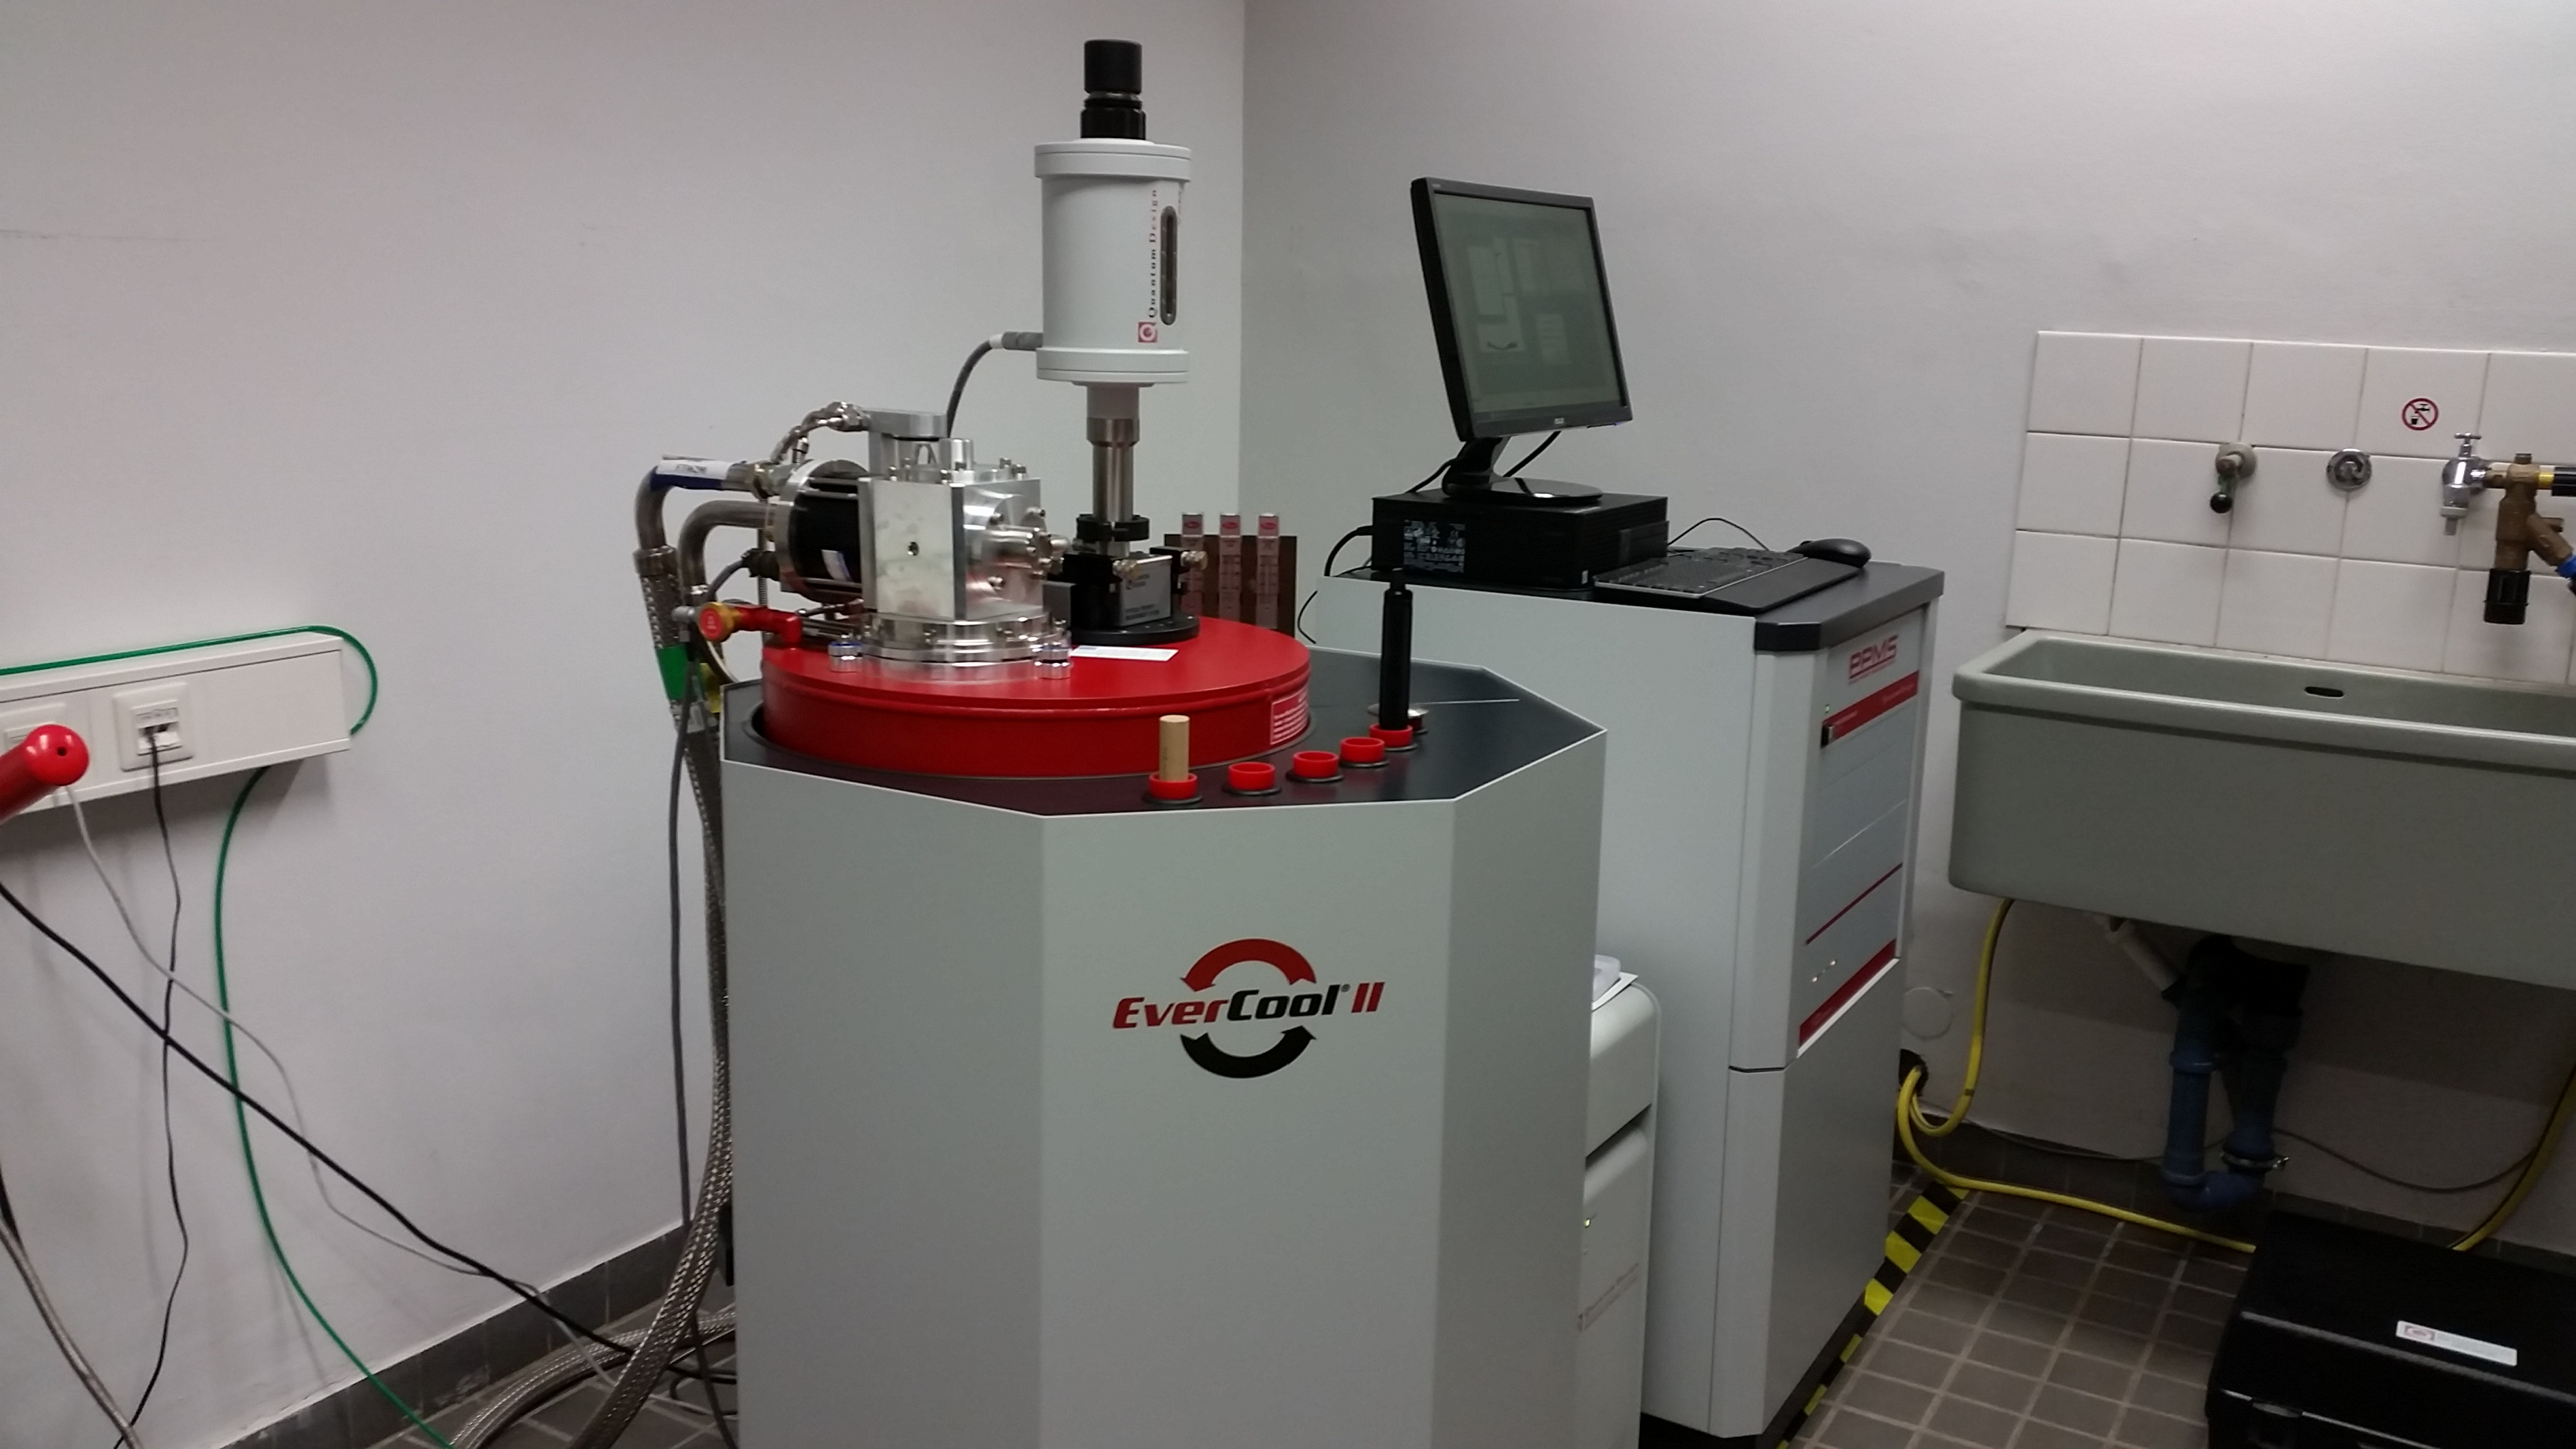
\includegraphics[width=0.7\textwidth]{instruments_ppms}
  \caption{\label{fig:appendix:instruments:ppms}Physical property measurement system (PPMS) Evercool II. The instrument is used to measure macroscopic magnetization properties.}
\end{figure}
The macroscopic magnetization of a sample can be measured by using Faraday's law of induction
\begin{align}
  U \eq \frac{\dint }{\dint t} \Phi,
\end{align}
which relates the voltage measured between the two ends of a wire loop with the change of the magnetic flux that passes through the wire with respect to time.
The magnetic flux $\Phi \eq B A$ is given here by the product of the magnetic field times the area that is enclosed by the wire loop.
Vibrating sample magnetometry uses this fundamental principle of electrodynamics to measure the magnetization by placing a small magnetic sample into a homogeneous field $B$ and vibrate it periodically with a small amplitude and defined frequency.
The periodic movement of the magnetic sample results in a slight periodic change of the magnetic field that passes through pickup coils placed around the sample and therefore in a periodic voltage that can be measured and enhanced by a lock-in amplifier.
The lock-in amplifier filters the specific frequency by multiplying the electric signal with a second signal of the same frequency using that
\begin{align}
  \sin(\omega t) \sin(\omega t) \eq \frac{1}{2} \biggl( 1 - \cos (2 \omega t) \biggr).
\end{align}
another freq

\section{Bruker D8 - X-Ray Reflectometry}
\label{app:additionalExperimentalTechniques:xrr}
\begin{figure}[h]
  \centering
  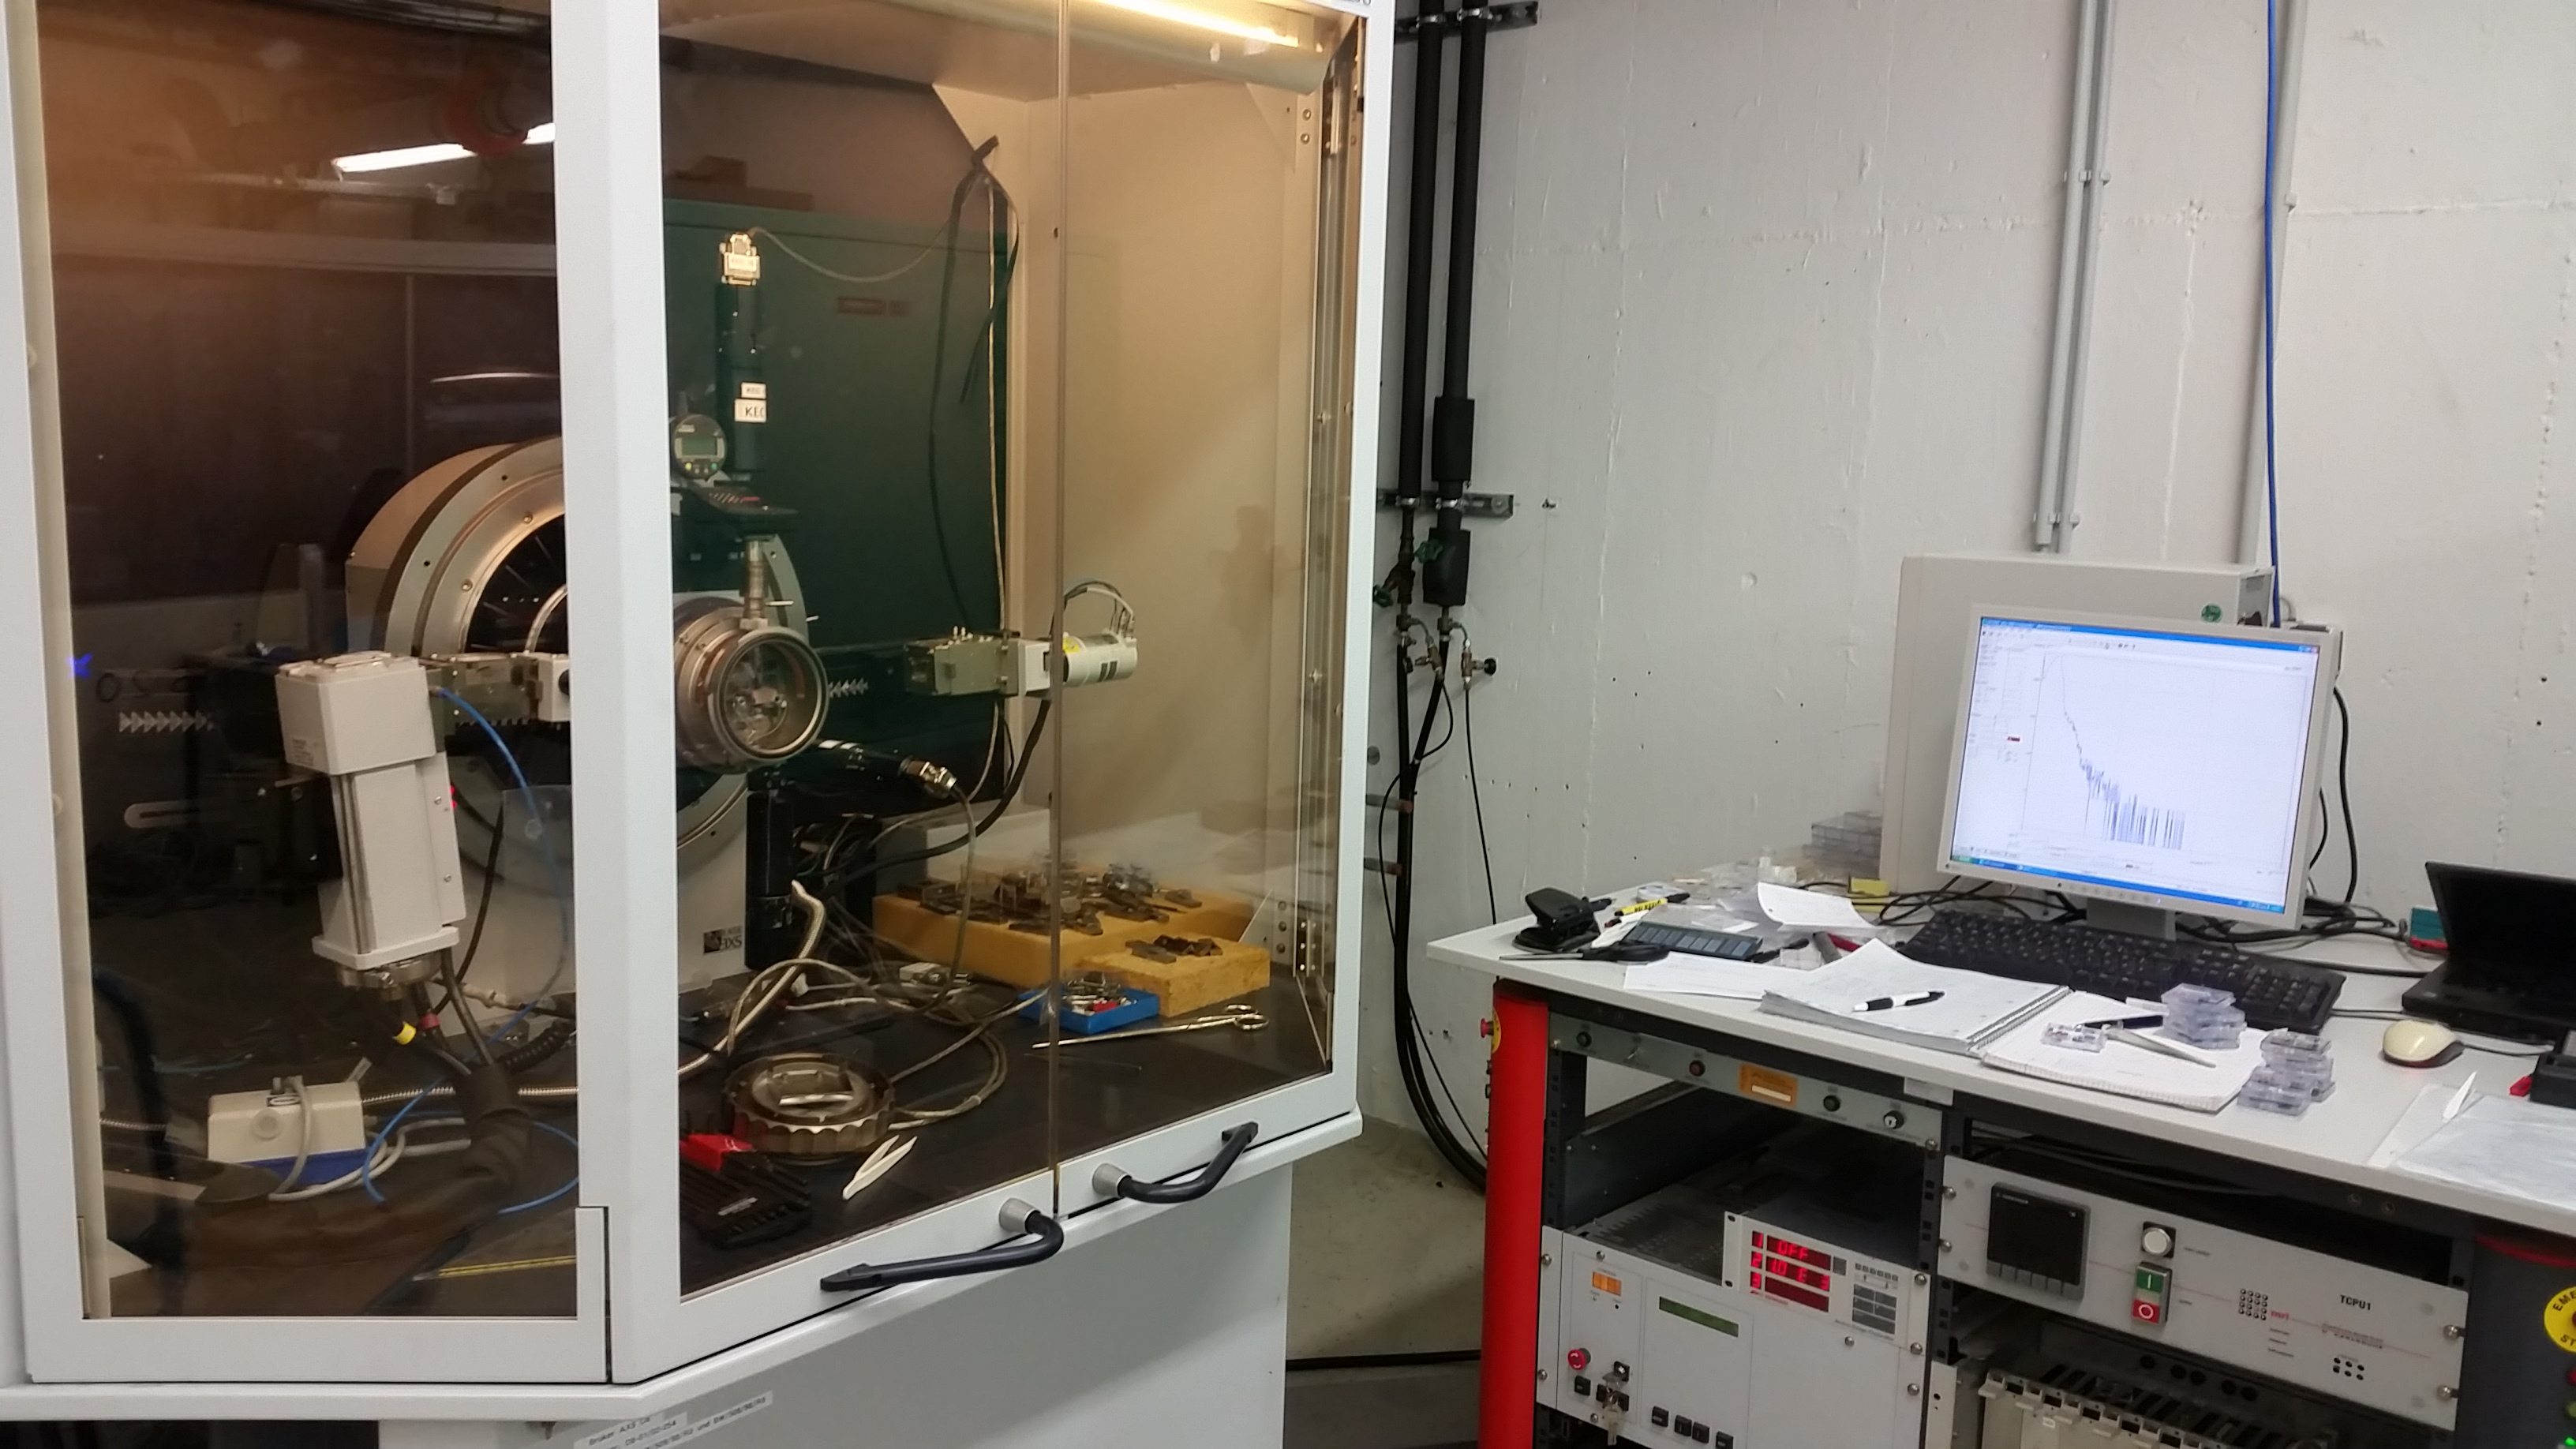
\includegraphics[width=0.7\textwidth]{instruments_brukerD8}
  \caption{\label{fig:appendix:instruments:brukerD8}Bruker D8 instrument which can be used for x-ray reflectometry and x-ray diffraction.}
\end{figure}
To study the vertical structure of thin-layer samples, x-ray reflectometry (XRR) is a quick method. In this work, multiple samples were studied with XRR using the \textsc{Bruker D8} instrument in the \textsc{Forchungszentrum J\"ulich}.
For XRR, the incident angle of the beam and the outgoing angle are increased simultaneously to maintain the specular condition while scanning the reflected intensity over $q_z$.
The beam size can be varied by slits and is typically set to $0.2 \unit{mm}$.
To estimate the beam divergence, the direct beam is scanned with the detector in \reffig{fig:appendix:instruments:brukerD8DirectBeam}.
The best fit with a gaussian function results in a divergence of $\Delta \alpha_i \eq 0.01510(4) ^\circ \eq 2.635(7) \cdot 10^{-4}.$
\begin{figure}[h]
  \centering
  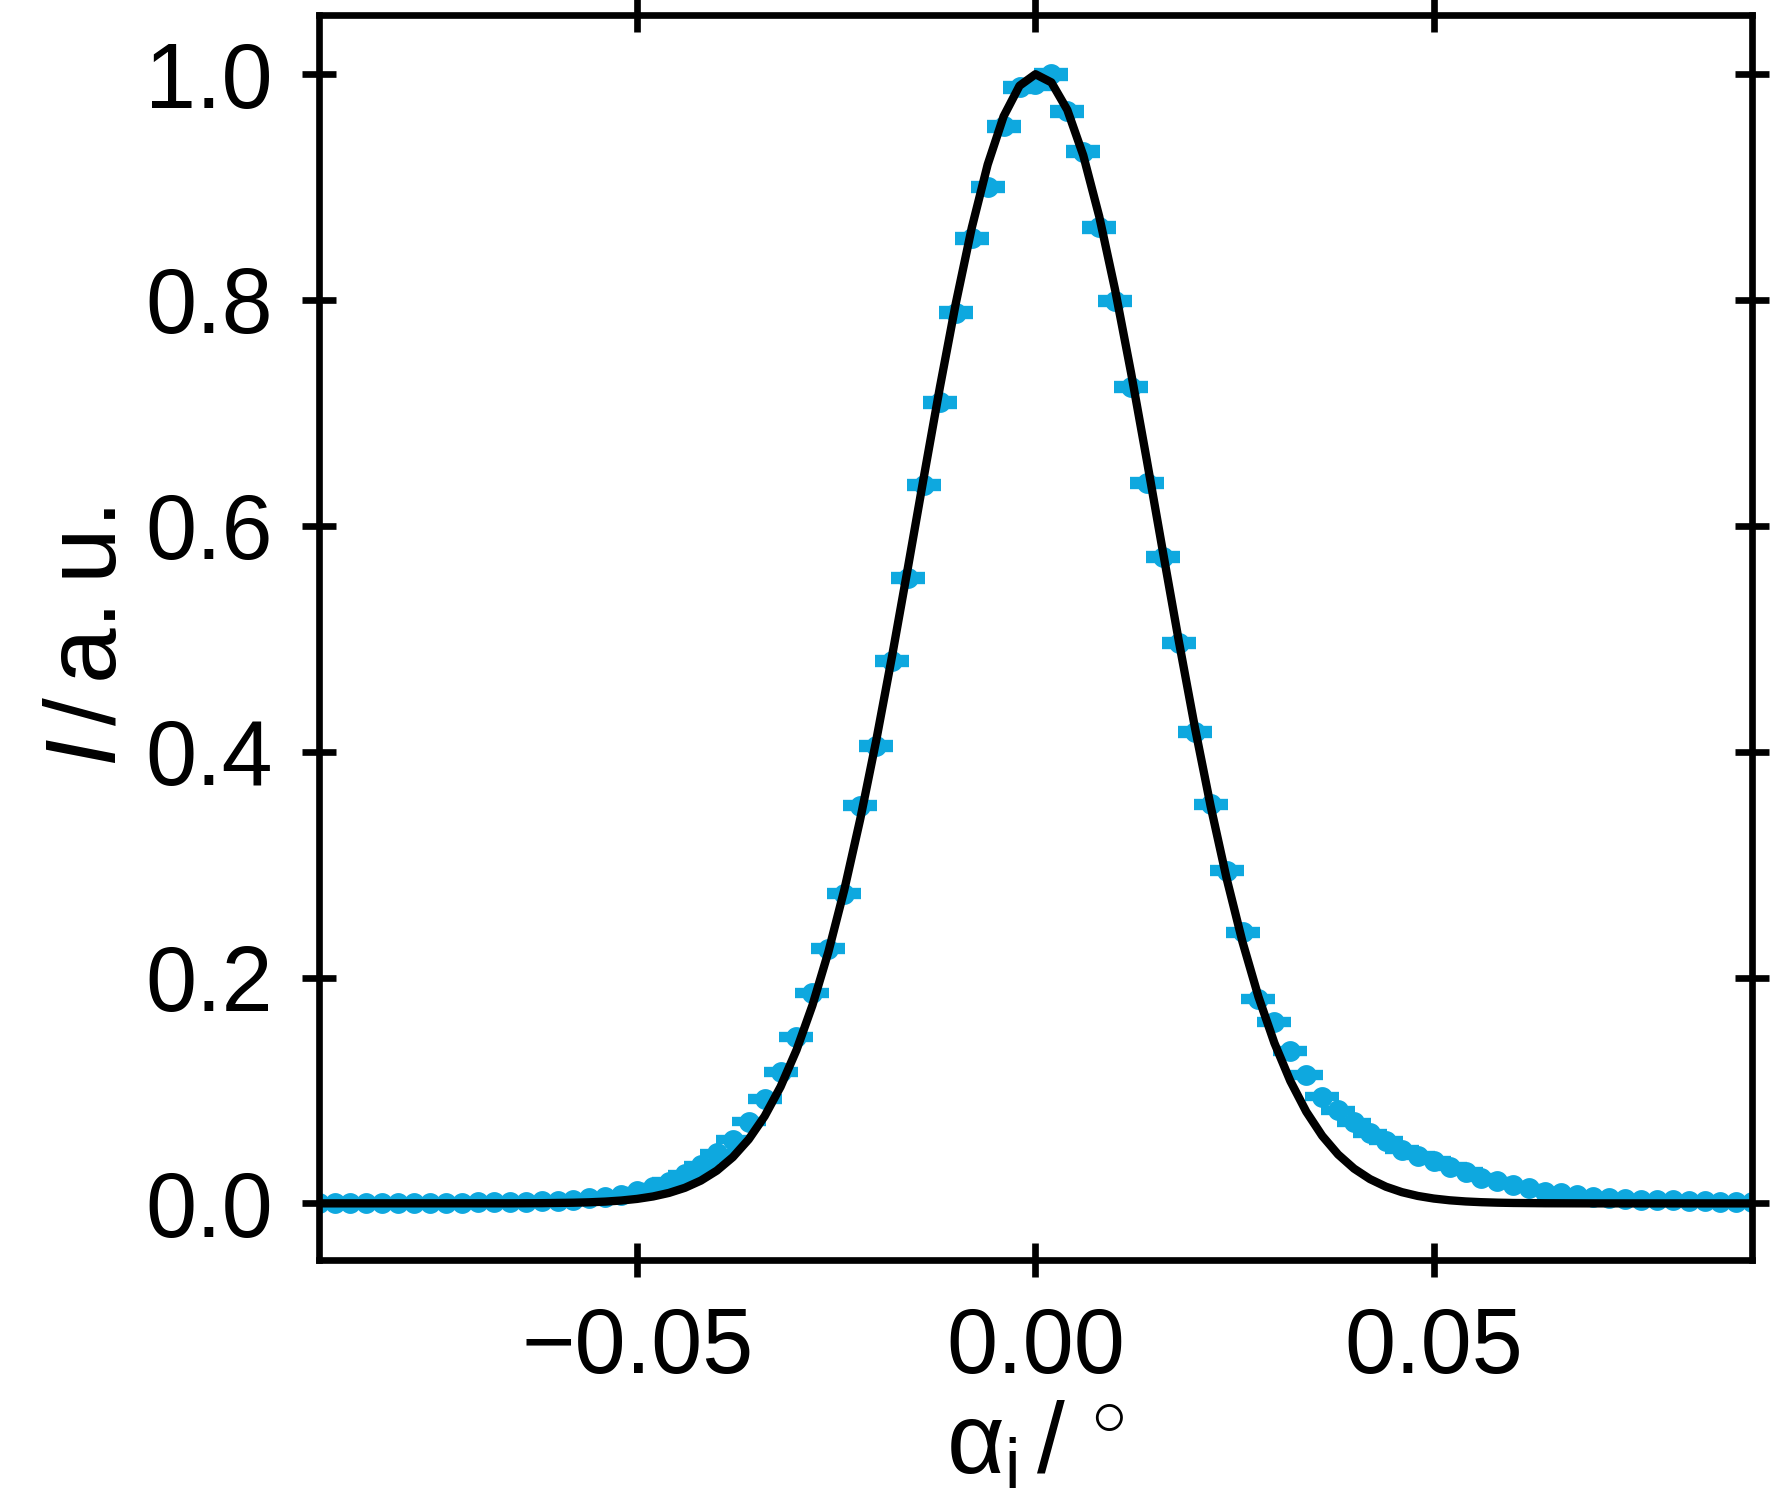
\includegraphics{appendix_instruments_brukerD8DirectBeam}
  \caption{\label{fig:appendix:instruments:brukerD8DirectBeam}Direct beam scan of the Bruker D8 instrument at a beam slit size of $0.2 \unit{mm}$, modelled by a gaussian function to estimate the divergence.}
\end{figure}

\section{Neon Zeiss 40 - Scanning Electron Microscopy}
\label{app:additionalExperimentalTechniques:sem}
\begin{figure}[h]
  \centering
  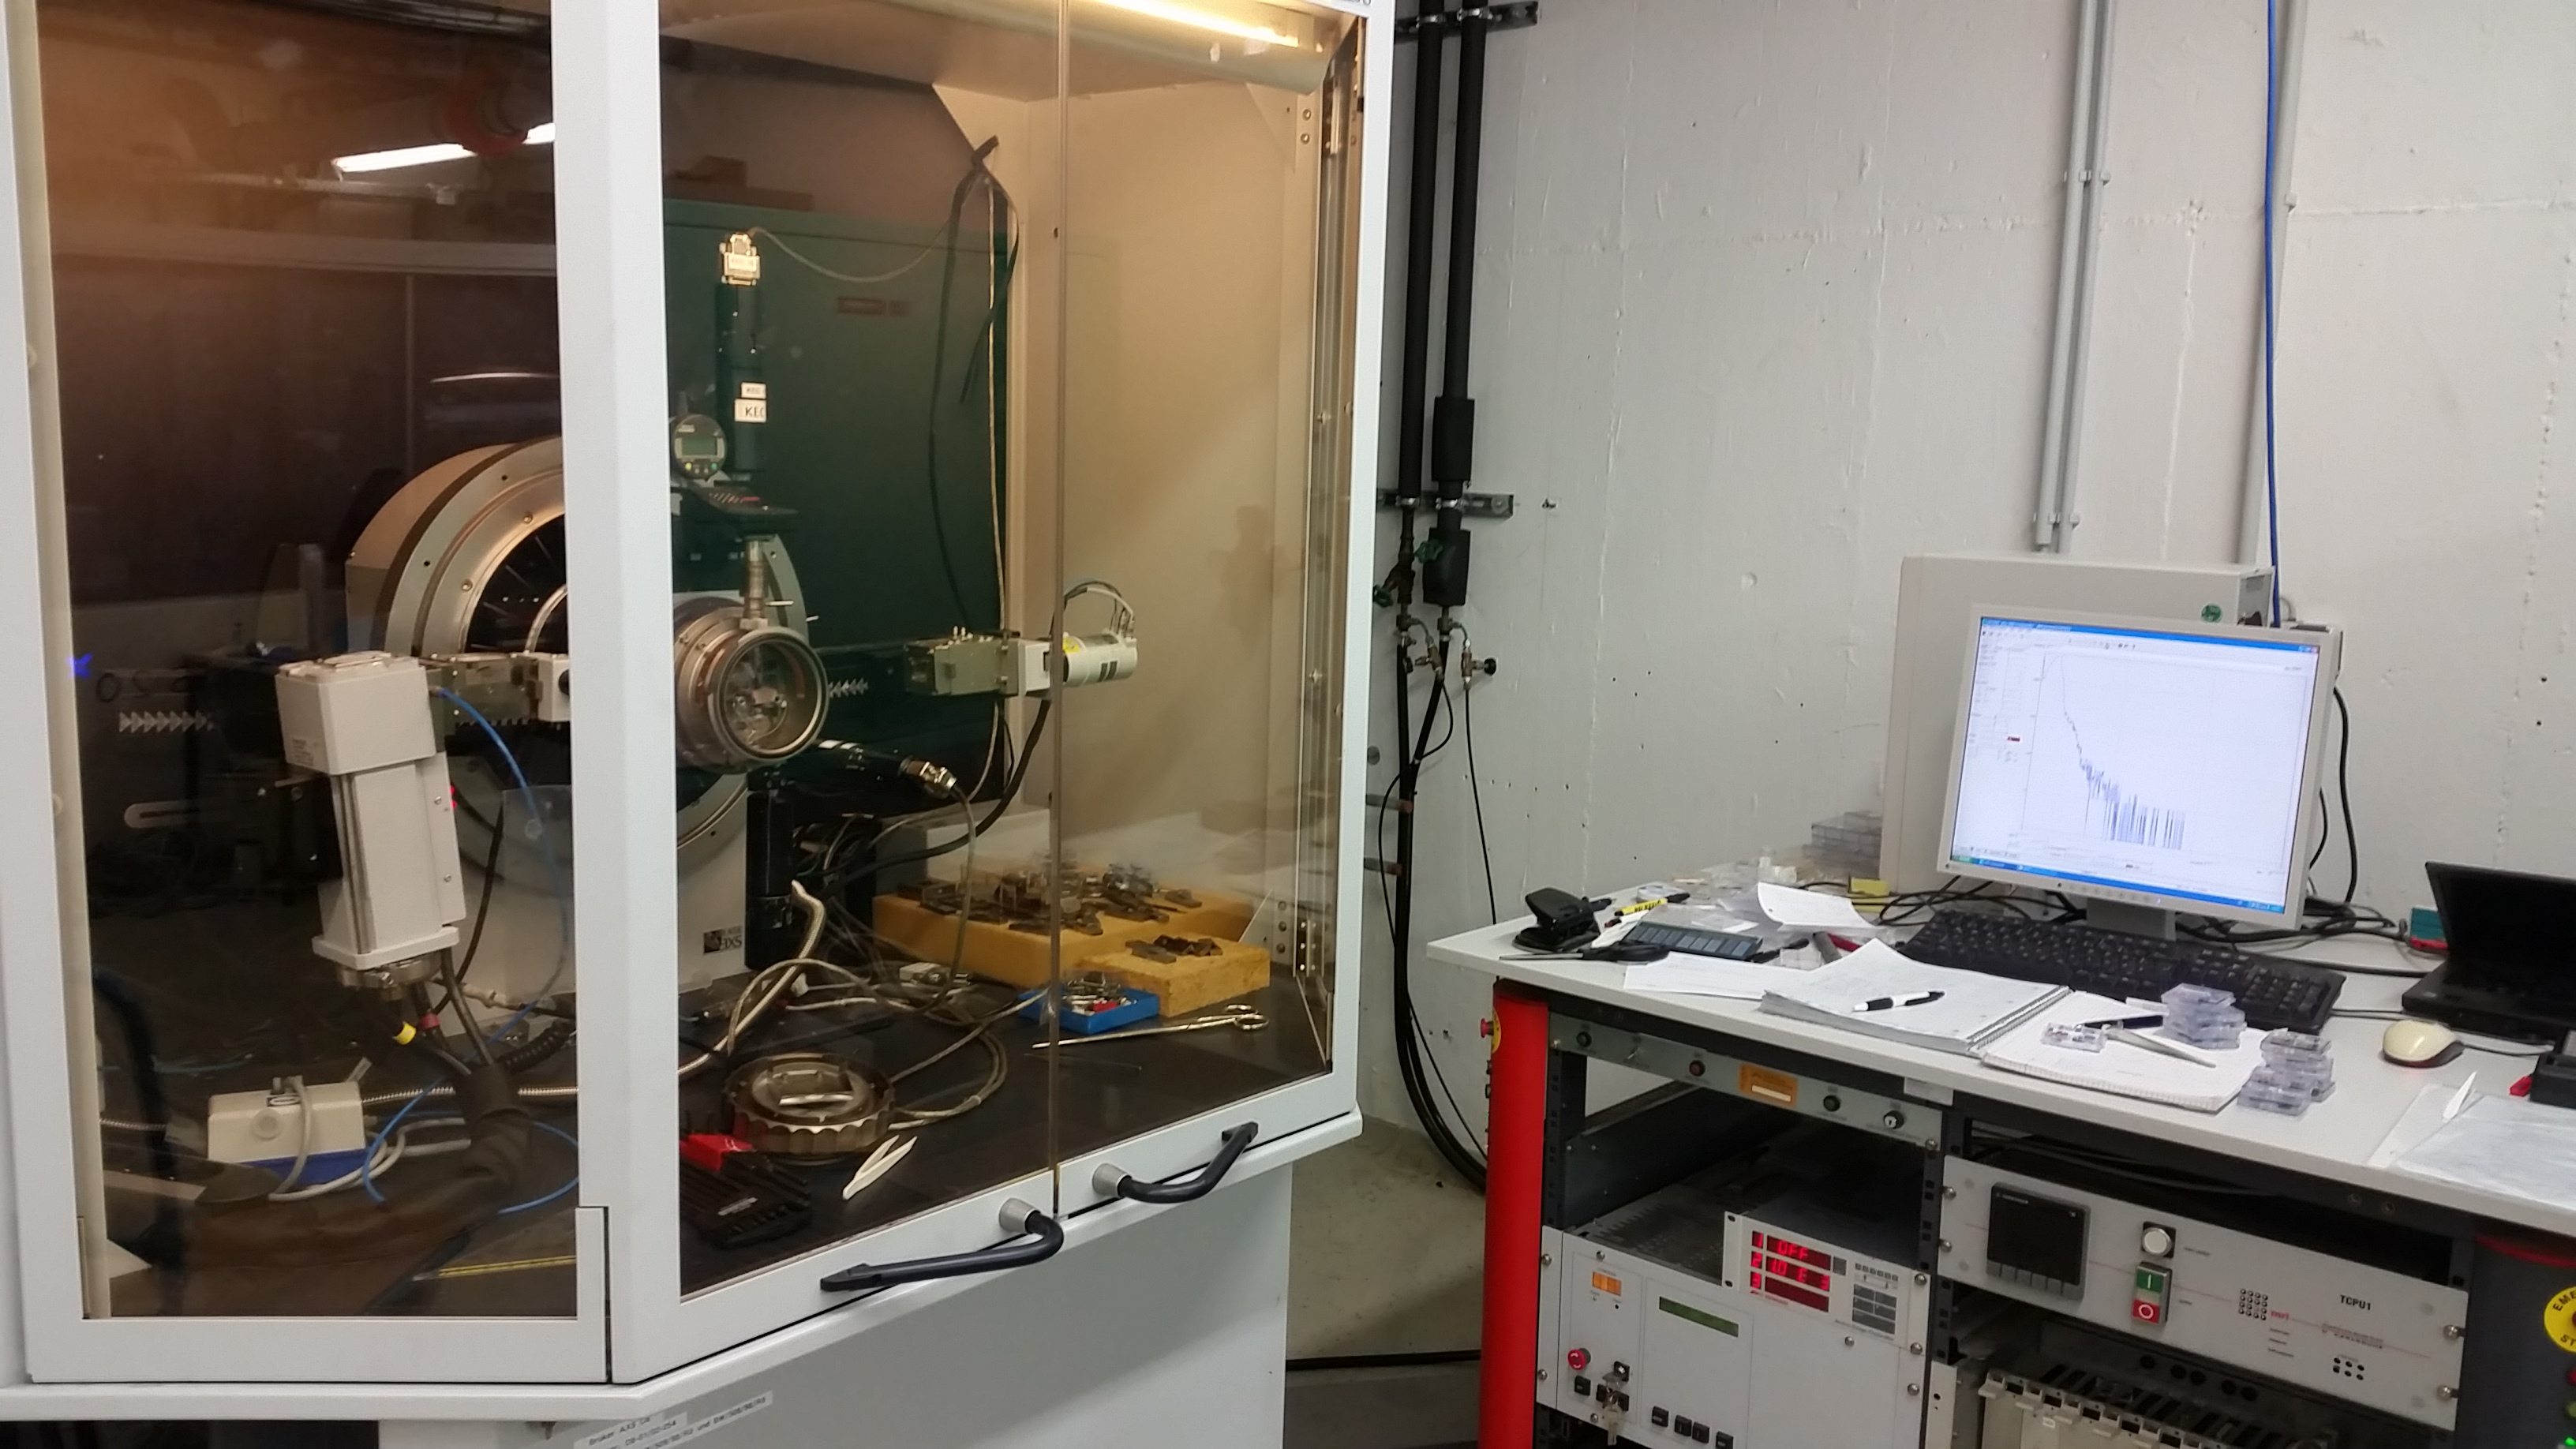
\includegraphics[width=0.7\textwidth]{instruments_brukerD8}
  \caption{\label{fig:appendix:instruments:brukerD8}Bruker D8 instrument which can be used for x-ray reflectometry and x-ray diffraction.}
\end{figure}

\end{document}
